\section{Introduction} \label{sec:intro}
Social microblogs such as Twitter and Weibo are experiencing explosive growth, with billions of users globally sharing their daily status updates online.
For example, Twitter has more than 255 million average monthly active users (78\% from mobile) as of March 31, 2014, and an estimated increase of 25\% per year\footnote{http://solomozone.com/tag/revenues/}.
Various studies have shown that Twitter is viable as a social ``sensor'', and holds great promise for detecting and forecasting significant societal events~\cite{bugel2013multilingual,sakaki2010earthquake}.
In recent years, a significant body of research~\cite{aggarwal2012event,hong2012discovering,lappas2009burstiness,lappas2012spatiotemporal,sakaki2010earthquake,sayyadi2009event,watanabe2011jasmine,weng2011event,yin2011geographical} has focused on modeling bursts and increases of user activity in social media.

However, real world events are not only correlated with burst signals, but can also exhibit unusually low levels of activity in social networks.
As shown in Figure 1, a protest in the city of Natal, Brazil began at 5:00 PM (local time) at the Museum of the Republic, with people gradually joining the demonstration. %\footnote{http://www.jb.com.br/pais/noticias/2013/06/17/manifestantes-invadem-cobertura-do-congresso-nacional-em-brasilia/}.
On Twitter, there was an uncharacteristic lull in activity or {\it group absenteeism} behavior from 6:00 PM---8:00 PM on the same day.
%Another example comes from December 24, 2013, southern Brazil experienced widespread flash floods. According to news sources, more than 50,000 people were forced to flee their homes in Minas Gerais and Espirito Santo, in the southern states of Brazil. Immediately following the floods, Twitter activity in this region dropped by 51\%, and reached its lowest point that evening.
%Other examples of \textit{group absenteeism} that we observed from Latin American Twitter activity include bus strikes in Brazil on May 21, 2014, the Iquique earthquake in Chile on April 1, 2014, and a major power supply disruption in Argentina on December 30, 2013.



\begin{figure}[t]
\centering
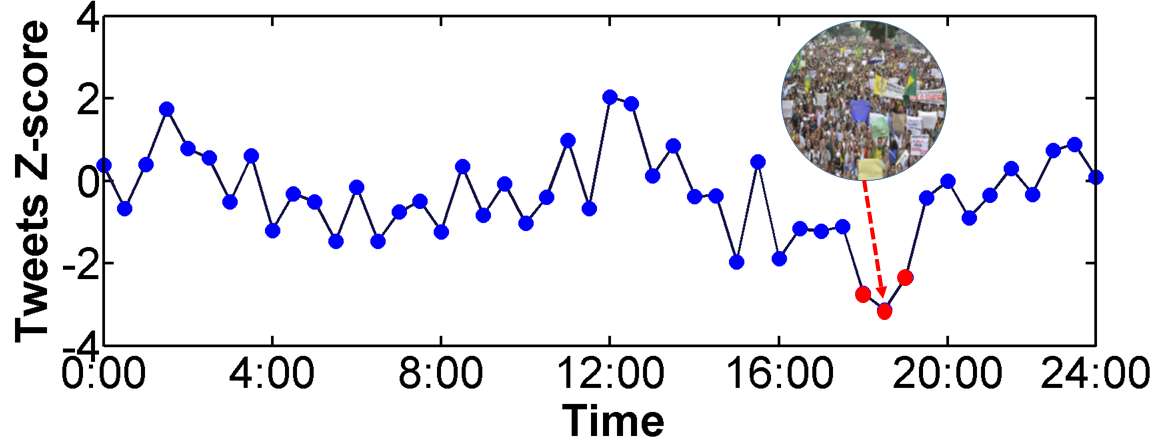
\includegraphics[width=4.5in]{figures/Natal_example1.png}
\caption{Detected group absenteeism in Natal, Brazil beginning at 6:00 PM on June 17, 2013. This absenteeism event coincides with a large protest that happened in the region.}
\label{fig:natal-protest}
\end{figure}


Investigating this phenomenon of unusually calm behavior online holds enormous potential for understanding localized, disruptive societal events.
In this paper we focus on absenteeism based event detection, and introduce this important topic as a key data mining
task for social media analytics.
An \textit{absenteeism} event in social networks can be defined as an event which is characterized by a significant lull in activity such as a sudden, sharp decrease of Twitter volume within a short period of time (and which  often precedes a major burst in re-activity).
This paper presents the first study to systematically investigate group absenteeism in LBSNs.
Using graph wavelet techniques, we pose this problem as one of group anomaly detection.
To appropriately incorporate absenteeism concepts into our detection approach, we must first address the following questions:

\begin{itemize}
\item What scale should we select to model the absenteeism groups? %Which node should be the central point?
    
\item What is the most efficient approach to select absenteeism groups that are spatially and temporally localized?
    
\item How do we model an absenteeism signal for event detection? Even though we have clear examples of real world events which can explain the observed absenteeism, not all absenteeism occurrences can be associated with underlying events. Therefore we must be able to differentiate absenteeism from noisy signals for event detection.
\end{itemize}

Graph wavelets display two outstanding advantages to study the above
questions: scalability and low computational complexity.
In this scenario, the data objects are embedded in a general graph as vertices.
By employing wavelet transforms on the graph, we can construct a wavelet function with a graph structure, and we are able to select absenteeism groups at different scales.
Lastly, we propose a two-pass group anomaly detection method that first detects absenteeism, and then checks if there is a subsequent burst in activity within a specific time period.
By comparing correlations between the wavelet coefficients of both of these groups, we are able to relate observed absenteeism to a possible real world event.

Our contributions are thus:

\begin{itemize}
\item To the best of our knowledge this is the first study to modeling group absenteeism as a basis for event detection.
%Even though burst has been extensively discussed in previous work, however, the absenteeism has different patterns and plays an irreplaceable role in event detection.

\item We incorporate graph wavelets as a mechanism to detect the most anomalous subgraphs at different scales. We demonstrate how this is a powerful technique for social media analytics.

\item We propose a novel two-pass event detection method that uses correlation scores between the group depicting \textit{absenteeism} and the group demonstrating increased activity to probabilistically determine the likelihood of an event.
\end{itemize}

The rest of the paper is organized as follows. Section~\ref{sec:related} reviews related work and existing methodologies and Section~\ref{sec:preliminaries} formalizes the research problem. In Section~\ref{sec:algorithm}, we first discuss the graph wavelet formalism for group absenteeism detection, and subsequently demonstrate how it can be used for two-pass event detection. Section~\ref{sec:experiment} presents extensive experiments for event detection, and the paper concludes with a summary of the research in Section~\ref{sec:conclusion}.



%\begin{itemize}
%\item How do we differentiate absenteeism from noise signals?
%\item How can wavelet graph be used for group abnormality detection?
%\item How do we detect events from linking absenteeism group with burst group?
%\end{itemize}
